\documentclass[
    prb,altaffilletter,citeautoscript,
    amsmath,amssymb,
    showpacs,showkeys,floatfix,
    reprint
    % preprint,linenumbers
    % come si ammazza il tempo? ... colpendolo
]{revtex4-1}
\usepackage{custom}
\usepackage{tikz}
\usetikzlibrary{optics}
\usepackage[varvw]{newtx}
\usepackage{esint}

\begin{document}

\title{Amplificatore lock-in per la misura dei coefficienti di Fresnel su cristalli non dielettrici}

\author{Francesco Polleri}
\email{s5025011@studenti.unige.it}

\author{Mattia Sotgia}
\email{s4942225@studenti.unige.it}

\affiliation{Università di Genova, Dipartimento di Fisica}
\date{\today}
\keywords{Amplificatori \textsc{lock-in}, strumenti di misura, equazioni di Fresnel, ellissometria.}

\begin{abstract}
    Presentiamo la progettazione e la realizzazione di un esperimento per la misura dei coefficienti di Fresnel di un film sottile di cristallo di Silicio (c-Si) e di un sottile campione di oro (Au). La misura è effettuata sfruttando un sistema di accoppiamento di fase \textsc{lock-in}\cite{scofieldFrequencydomainDescriptionLockin1994} che permette una migliore reiezione in frequenza del rumore. Descriviamo la progettazione del sistema di misura e infine una descrizione e discussione dei risultati confrontando con modelli teorici. Il sistema descritto permette di effettuare misure con sufficiente precisione dei coefficienti di Fresnel $R_s$ e $R_p$, permettendo di ottenere i coefficienti di riflessione e trasporto $n_\text{c-Si}/\kappa_\text{c-Si}$ e $n_\text{Au}/\kappa_\text{Au}$. Per il cristallo di silicio (c-Si) possiamo anche inferire il valore dello spessore del film di ossido di silicio ($\mathrm{SiO_2}$) depositato sul substrato di silicio. I risultati ottenuti sono molto complicati da interpretare, nonostante la estrema precisione del sistema, per la ridotta possibilità di controllare accuratamente il sistema ed eventuali fonti di errore e quindi i risultai sono di fatto per la maggior parte inconcludenti.
\end{abstract}
\maketitle

\let\tocname\relax
\tableofcontents

\section{Introduzione} 

L'utilizzo di un sistema sensibile allo sfasamento, come un amplificatore \textsc{lock-in}, può risultare molto comodo in applicazioni di misura in cui si fa utilizzo di segnali luminosi, in particolar modo se questi segnali sono periodici. In questo modo è infatti possibile ridurre sufficientemente i disturbi e le interferenze prodotte dal rumore esterno, che in un ambiente di laboratorio possono essere molteplici, e inoltre permette anche di controllare e ridurre fonti di rumore che sono invece causate dal sistema stesso e che sono di carattere aleatorio. Poiché il processo di lock-in consiste matematicamente nello spostare in frequenza un segnale, questo allora può anche essere utilizzato anche con segnali che sono teoricamente continui, modulandoli con un segnale a frequenza definita o nota, in modo da spostarli nello spettro in una regione a minore rumore, e poi riportandolo alla frequenza di partenza, rimodulando il segnale fisico con un riferimento in fase. Considerando allora un sistema che permette di generare e di acquisire con una frequenza definita, possiamo infatti ridurre molti di questi contributi di rumore, e quindi incrementare il rapporto tra segnale e rumore (SNR). 

Nel caso specifico della misura che vogliamo compiere il segnale è effettivamente un segnale in continua, dato da una sorgente coerente di luce sufficientemente collimata. Questa viene polarizzata e fatta incidere sul campione cristallino che la riflette. Il segnale riflesso è quello che poi viene acquisito. Trovandosi a bassissima frequenza il segnale è però estremamente soggetto a rumore. Se infatti studiassimo il segnale del laser in continua questo presenterebbe distorsioni legate al comportamento sub-ottimale a basse frequenze, dove la maggior parte delle fonti di rumore sono presenti. Per evitare tali distorsioni allora spostiamo il segnale in frequenza in una regione dello spettro con un migliore SNR. La soluzione allora è individuabile nel spostare il segnale da $\nu=\SI{0}{\Hz}$ ad una frequenza che sia in una regione dello spettro il più possibile a basso rumore. Il passo successivo è convertire il segnale in continua sfruttando l'accoppiamento in fase con un riferimento e infine riportare il segnale alla stessa frequenza di partenza. 

Questo sistema così progettato può essere allora utilizzato per effettuare misure dei coefficienti di Fresnel\cite{fresnelCalculationTintsThat2021,fresnelNoteCalculTeintes1821} $r$ e $R$ dati differenti campioni di cristalli, conduttori elettrici. L'obiettivo scientifico è quindi quello di poter caratterizzare le curve di Fresnel per i coefficienti di riflessione per i due campioni e nel farlo studiare anche il comportamento dell'amplificatore \textsc{lock-in}. 

Il documento è diviso in una parte immediatamente successiva che descrive a grandi linee alcune formalizzazioni del sistema utilizzato a cui segue poi un dettaglio sulla teoria fisica del fenomeno studiato per definire al meglio le osservabili in questione e infine una descrizione e caratterizzazione dell'esperimento con una breve discussione sulle modalità di analisi dati e sui risultati ottenuti. 

\paragraph*{Teoria del lock-in} 
Il segnale fisico (nel caso specifico il segnale è dato dal fascio luminoso) è modulato su un'onda sinusoidale\footnote{Nel caso sperimentale il segnale è modulato su un'onda quadra, essendo utilizzato un \emph{chopper}, ma la matematica si complicherebbe, riportiamo quindi eventuali correzioni alla teoria generale nelle note.} come $V_0 \cos(\omega_\mathrm{r} t)$, dove il pedice r indica che si tratta anche della frequenza con cui andiamo poi a stimolare il riferimento che forniamo al \emph{lock-in}. $V_0$ è l'ampiezza del segnale fornita al sistema. 

Il sistema complessivo avrà allora un output della forma $V_\mathrm{out} \cos(\omega_\mathrm{r} t + \phi_\mathrm{out}),$ dove una fase arbitraria, ma non casuale, può essere in generale aggiunta dal processo fisico che stiamo studiando. Il segnale di riferimento fornito in ingresso al \textsc{lock-in} allora deve anche esso presentare una fase $\phi_\mathrm{ref}$ per fare in modo che sia accoppiato al segnale che viene letto dal rivelatore. 

Il segnale fisico che allora avremo in ingresso al \textsc{lock-in} è dato da un primo stadio di amplificazione, che compie l'operazione \begin{equation}
    V_\mathrm{out} \cos(\omega_\mathrm{r} t + \phi) \to s_\mathrm{in}(t) = G_\mathrm{amp}V_\mathrm{out} \cos(\omega_\mathrm{r} t + \phi),
\end{equation} dova anche un eventuale rumore $n(t)$ viene portato in $G_\mathrm{amp}n(t)$. Successivamente all'accoppiamento in fase avremo il prodotto tra $s_\mathrm{in}(t)r(t)$, con $r(t)$ il riferimento fornito dopo lo stadio di amplificazione. Come riportato in ref. \onlinecite{scofieldFrequencydomainDescriptionLockin1994}, dopo un ultimo stadio passa-basso ottenuto con un filtro LPF (\emph{Low Pass Filter}), il sistema avrà ridotto notevolmente le componenti di rumore casuali, ma resterà ancora caratterizzato dalle componenti sistematiche del rumore \begin{equation}
    s_\mathrm{LPF}(t) = \frac{G V_\mathrm{out}}{2} \cos(\phi) + \frac{G \eta(\omega_0)}{2}\cos(\phi_\mathrm{n}(\omega_0)), \label{eq:s_LPF}
\end{equation} dove indichiamo con $\eta(\omega_0)$ la componente di rumore che corrisponde alla frequenza a cui sta operando il sistema \textsc{lock-in}, che non può essere eliminata automaticamente, ma può essere ridotta scegliendo una precisa regione nel dominio delle frequenze dove sappiamo che abbiamo meno rumore (evitiamo ad esempio di scegliere come frequenza di modulazione la $\SI{50}{\Hz}$).

Per questa breve introduzione abbiamo trascurato di trattare un segnale di riferimento che non è sinusoidale ma può essere ad esempio un'onda quadra. Questa spettralmente presenta non solo un picco principale, ma introduce anche armoniche successive a quella principale $\omega_0$, che implicano la necessità di una migliore calibrazione del sistema. Per questo la frequenza di operazione del \textsc{lock-in} $\omega_0$ dovrà essere calibrata assieme alla frequenza di taglio del LPF per tagliare con maggiore efficienza le armoniche a frequenze più alte.  

Un altro termine su cui abbiamo controllo è infine la differenza di fase $\phi_\mathrm{out} - \phi_\mathrm{ref} = \phi$ della \eqref{eq:s_LPF}, dove osserviamo inoltre che massima efficienza per il sistema si ottiene per $\phi\ll 1$, per cui $\cos\phi\simeq1$.

\section{Teoria}

Prima di presentare la progettazione e caratterizzazione del sistema procediamo a definire con un po' più di rigore la misura che vogliamo effettuare e la teoria sottostante. 

Considerato un fascio di luce generico ogni possibile angolo di polarizzazione è espresso dalla combinazione lineare di due vettori di una base di polarizzazione, che possono essere scelti in modo da essere ortonormali, posto uno parallelo, denotato da $p$, e l'altro ortogonale al piano di incidenza, denotato da $s$. Queste due polarizzazioni prendono anche altre definizioni, per esempio descrivendo quale campo è ortogonale al piano di incidenza. Avremo allora che onde polarizzate $p$ sono anche definite \emph{transverse-magnetic} (TM), e onde polarizzate $s$ sono definite \emph{transverse-electric} (TE). La percentuale di luce riflessa, dato un campione di materiale X, è dipendente dal grado di polarizzazione ed espressa dalle relazioni ottenute da Fresnel\cite{fresnelCalculationTintsThat2021,fresnelNoteCalculTeintes1821}, per cui avremo che il coefficiente di riflessione per onde TE è dato come \begin{equation}
    r_\mathrm{s} = \frac{\underline{n}_1\cos\theta_i - \underline{n}_2\cos\theta_t}{\underline{n}_1\cos\theta_i + \underline{n}_2\cos\theta_t} = \frac{\underline{n}_X\cos\theta_i - \underline{n}_2\cos\theta_t}{\underline{n}_X\cos\theta_i + \underline{n}_2\cos\theta_t},
    \label{eq:fresnel_rs}
\end{equation} mentre per le onde TM è dato come \paragraph*{}\begin{equation}
    r_\mathrm{p} = \frac{\underline{n}_2\cos\theta_i - \underline{n}_1\cos\theta_t}{\underline{n}_2\cos\theta_i + \underline{n}_1\cos\theta_t} = \frac{\underline{n}_2\cos\theta_i - \underline{n}_X\cos\theta_t}{\underline{n}_2\cos\theta_i + \underline{n}_X\cos\theta_t}. 
    \label{eq:fresnel_rp}
\end{equation} In generale il coefficiente $n_1=n_\mathrm{X}$ indica il coefficiente di rifrazione del materiale che si sta considerando. Tale coefficiente è generalmente reale, ma per materiali conduttori, si è osservata la necessità di estendere la teoria\cite{attwoodSoftXRaysExtreme1999} introducendo il coefficiente complesso $\underline n = n + i\kappa$, dove $\kappa$ e $n$ sono quantità caratteristiche del materiale in considerazione determinabili sperimentalmente. Generalizziamo allora le \eqref{eq:fresnel_rs} e \eqref{eq:fresnel_rp} considerando indici di rifrazione complessi. Questi sono allora effettivamente funzioni a variabile complessa. La frazione riflessa, detta riflettanza, è data allora da \begin{equation}
    R_\ell= \qty|r_\ell|^2, \quad \ell = \mathrm{s,p} \label{eq:R}
\end{equation} e tende a 1 per l'angolo di riflessione che tende a \SI{90}{\degree}.

Nelle relazioni \eqref{eq:fresnel_rs} e \eqref{eq:fresnel_rp} in realtà è possibile avere funzioni ad una sola variabile (che può essere sia $\theta_i$ che $\theta_t$, ma generalmente, con la scelta di poter controllare l'angolo di incidenza del fascio luminoso, si considera $\theta_i$) ricordando che dalle leggi di Snell \begin{equation}
    \cos\theta_t = \sqrt{1-\qty(\frac{\underline n_1}{\underline n_2}\sin\theta_i)^2}.
    \label{eq:snell}
\end{equation}

Questo modello è sufficientemente valido quando l'interfaccia che si sta studiando è semplice e il materiale su cui il fascio di luce è fatto incidere è sufficientemente profondo da disperdere al suo interno la maggior parte della radiazione incidente, senza avere quindi altri fenomeni di riflessioni secondarie. Questo è quindi lo consideriamo valido per il caso del campione di oro (fig. \ref{fig:Au}).

\begin{figure*}
    \centering
    \subfloat{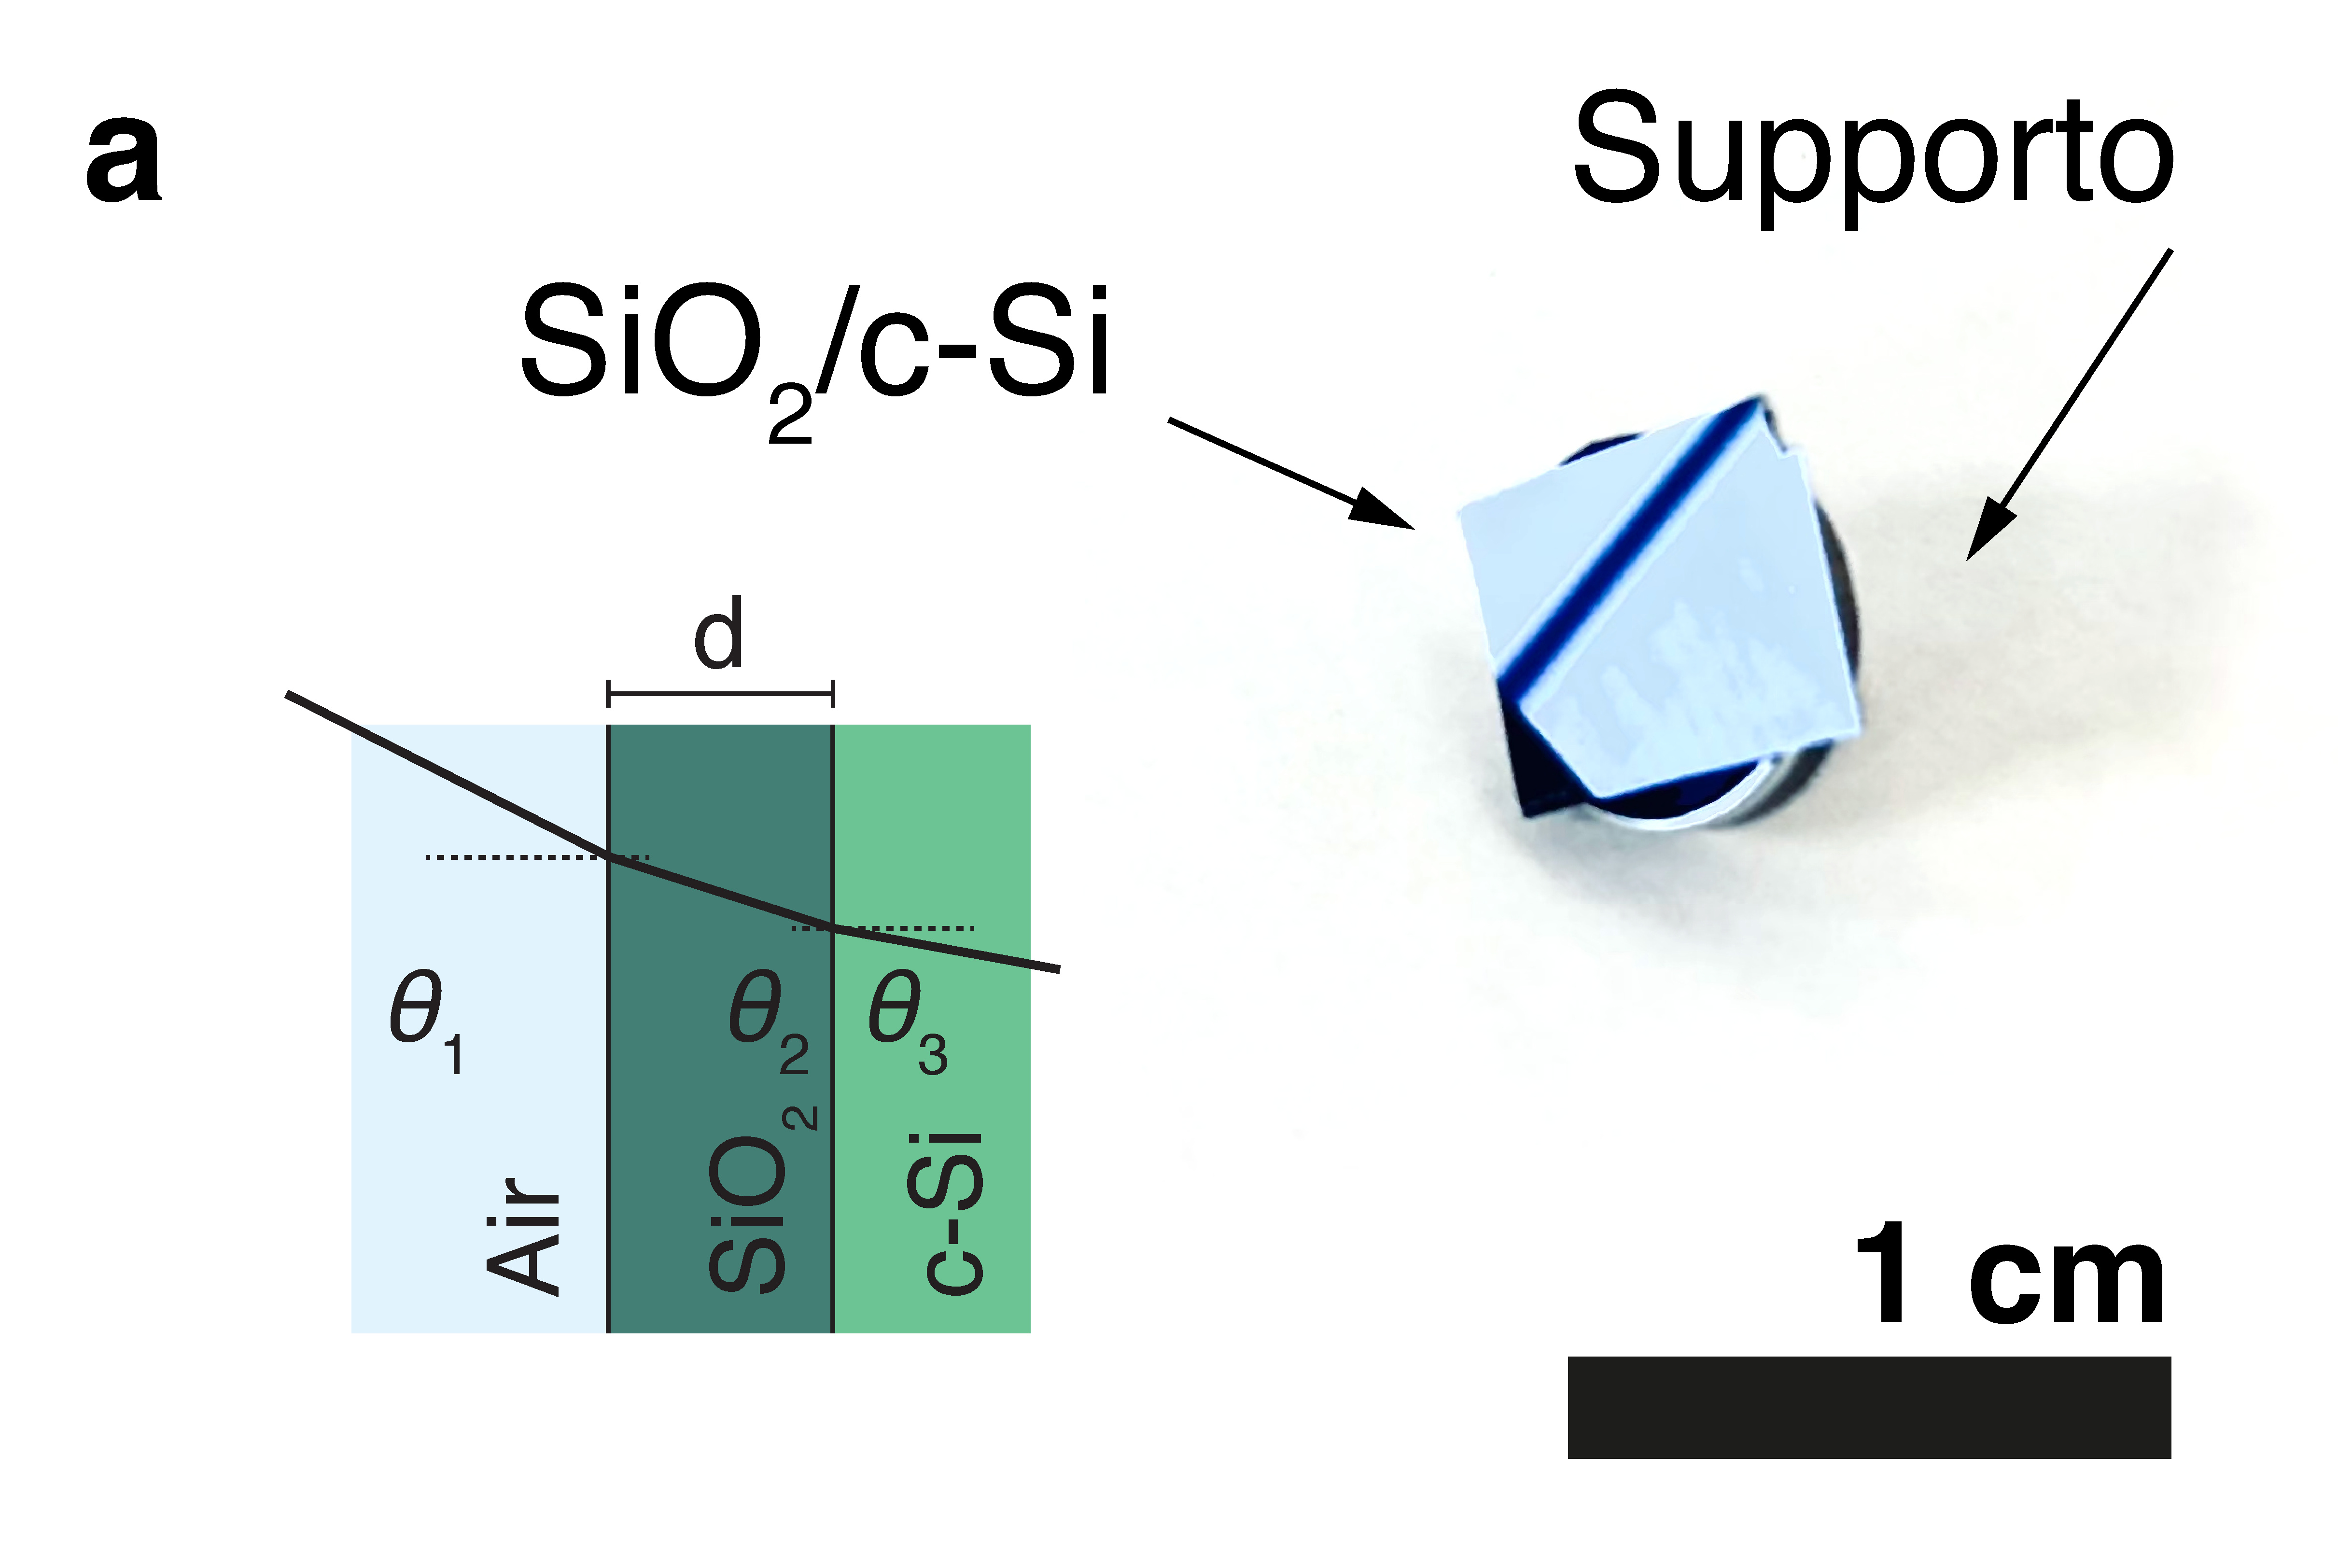
\includegraphics[width=0.4\linewidth,trim={0 4cm 0 0}]{figures/c-Si.pdf}\label{fig:c-Si}}
    \subfloat{\includegraphics[width=0.4\linewidth]{figures/Au_sample.pdf}\label{fig:Au}}
    \caption{\ref{sub@fig:c-Si} Campione di  cristallo di Silicio montato sul supporto necessario per poter effettuare le misure. A lato è anche schematizzata la struttura a layer dell'interfaccia del c-Si con l'aria, a cui è interposto un sottile strato di $\mathrm{SiO_2}$ che cambia quindi l'angolo con cui la luce incide sul silicio. \ref{sub@fig:Au} Campione di oro e schema della struttura dell'interfaccia aria/oro. Il campione è montato al centro del goniometro. Sullo stesso supporto è possibile anche fissare il campione di c-Si.}
    \label{fig:c-Si/Au_samples}
\end{figure*}

Ci possono essere però alcune situazioni in cui il modello semplificato non è sufficiente, sopratutto quando il materiale in questione, per quanto preparato con estrema precisione, presenta sottili strati superficiali di materiale con indice di rifrazione differente. Questo è vero in particolar modo per il cristallo di silicio, c-Si, per il quale si ha un deposito di ossido di silicio $\mathrm{SiO_2}$ (vedi figura \ref{fig:c-Si}) con uno spessore $\SI{1}{\nano\metre}<d<\SI{10}{\nano\metre}$ sufficiente per avere fenomeni di riflessione multipla nel sottile film interposto ad ambiente (aria, con indice di rifrazione noto, $n_\mathrm{Air}$) e il substrato di c-Si, con indice $\underline n_\text{c-Si}$. La teoria che ne segue si complica. Dobbiamo allora introdurre il modello a tre fasi\footnote{Nel caso della ref. {\onlinecite{yehOpticalWavesLayered1988}} la convensione sul segno dell'esponenziale è differente da quella utilizzata invece dalla ref. {\onlinecite{hinrichsEllipsometryFunctionalOrganic2018}}, ma questo è indifferente considerato che l'esponenziale complesso è periodico $2\pi$. Nella \eqref{eq:three_phase_model} utilizziamo la convenzione presentata nella seconda} (\emph{three-phases model}\cite{cobetEllipsometrySurveyConcept2018, hinrichsEllipsometryFunctionalOrganic2018, yehOpticalWavesLayered1988}) per cui i coefficienti introdotti in (\ref{eq:fresnel_rs}-\ref{eq:fresnel_rp}) non sono più sufficienti, ma dobbiamo introdurre i coefficienti \begin{equation}
    r_\ell = \frac{r_{al, \ell} + r_{ls, \ell}e^{2i\beta}}{1 + r_{al, \ell}r_{ls,\ell}e^{2i\beta}},\quad \ell = \mathrm{s,p}\label{eq:three_phase_model}
\end{equation} valida sia per i modi TE che per i modi TM di oscillazione. I coefficienti $r_{al}$ e $r_{ls}$ hanno la stessa forma di (\ref{eq:fresnel_rs}-\ref{eq:fresnel_rp}), considerando questa volta che però gli angoli di incidenza sono relativi all'interfaccia che si sta considerando: aria/$\mathrm{SiO_2}$ nel caso di $r_{al}$, e $\mathrm{SiO_2}$/c-Si nel caso di $r_{ls}$. Il coefficiente $\beta$ è invece indicativo della differenza di fase legata al cammino ottico all'interno del layer sottile depositato sulla superficie del cristallo (si veda l'eq. (1.16) di ref. \onlinecite{hinrichsEllipsometryFunctionalOrganic2018}), ed è espresso come \begin{equation}
    \beta = \frac{2\pi}{\lambda} d \sqrt{\underline n_l^2 - \underline n_a^2 \sin^2\phi_a}.\label{eq:beta_coeff}
\end{equation} Osserviamo subito che il modello è sicuramente più complesso del precedente, il che comporterà la necessità di fare assunzioni in fase di analisi dati per poter ottenere dei risultati con una trattazione semplificata. 

\section{L'esperimento}

Descriviamo nel suo funzionamento e nelle scelte di progettazione l'esperimento, concentrandoci prima brevemente sul sistema ottico utilizzato e poi sulle scelte riguardanti il funzionamento e le caratteristiche dell'amplificazione e acquisizione del segnale, che possiamo considerare come una prima analisi \emph{online} del dato ricevuto. Infatti dai differenti input che riceviamo possiamo passare poi ad un dato \emph{pulito} che è più facile maneggiare. 

Del sistema ottico andiamo a definire le tre componenti principali, quali la sorgente utilizzata, il campione con il relativo supporto e il ricevitore/trasduttore, che permette di acquisire segnali in tensione dal segnale fisico. 

Dell'analisi online invece definiamo gli stadi principali come sono riportati in figura \ref{fig:lock-in/block_diagram} e analizziamo le scelte di progettazione per assicurare il miglior funzionamento dell'esperimento. 

\subsection{Il sistema ottico}

\begin{figure*}
    \centering
    \subfloat{\includegraphics[height=5cm,page=1]{figures/setup.pdf}\label{fig:setup}}
    \subfloat{\includegraphics[height=5cm,page=2]{figures/setup.pdf}\label{fig:setup_on}}
    \caption{\ref{sub@fig:setup} Schema del setup utilizzato. $P_1$ è il primo polarizzatore, che controlla l'intensità del fascio, insiema a $P_2$, che inoltre permette di definire la polarizzazione della luce, ricordando che l'intensità dopo due filtri è proporzionale al $\cos\theta_{1,2}$ dell'angolo compreso tra i due filtri. \ref{sub@fig:setup_on} Fotografia dell'esperimento completo durante una misura. Si può facilmente vedere il sottile fascio laser in uscita dalla sorgente, che attraversa il disco del chopper e poi due lenti polarizzatrici. Il fotodiodo è pure visibile. Il campione è nascosto invece dal supporto posto al centro del goniometro. }
    \label{fig:setup_and_photo}
\end{figure*}

L'esperimento è costituito da un goniometro da banco ottico con precisione di \ang{0;20} su entrambi gli angoli (incidenza e riflessione) rispetto al campione posizionato al centro. Il goniometro è assicurato ad un banco ottico sfruttato come supporto per l'intero setup, controllato localmente da un computer con \textsc{LabView}, che permette anche l'acquisizione dei dati. Uno dei due bracci del goniometro ospita il supporto per la sorgente laser, mentre l'altro ospita il fotodiodo rivelatore. Sul cammino ottico del fascio di luce è inoltre inserito un modulatore in frequenza, immediatamente vicino alla sorgente e due filtri polarizzatori posizionati dopo il \emph{chopper} ma prima del campione al centro del sistema. Quello più lontano dalla sorgente è l'ultima lente che il fascio attraversa prima di incidere sul campione e definisce quindi il piano di polarizzazione dell'onda incidente. Quello immediatamente precedente è invece necessario per ridurre l'intensità della luce incidente sul campione e conseguentemente della frazione di luce che poi colpisce il fotodiodo per evitare una eccessiva usura del campione e dello strumento di misura e per evitare inoltre di avere un segnale con un'ampiezza eccessiva in ingresso sul sistema. La scheda di acquisizione è infatti limitata in ampiezza a circa \SI{10}{\volt}, per cui la scelta dell'angolo relativo tra le due lenti polarizzatrici è importante per poter controllare l'intensità secondo queste limitazioni sperimentali. Uno schema del setup utilizzato è in figura \ref{fig:setup}, mentre in figura \ref{fig:setup_on} troviamo una sua fotografia. 

\paragraph*{Sorgente} La sorgente è costituita da un laser verde estremamente collimato, alimentato in corrente continua. La luce emessa ha una lunghezza d'onda precisa e sufficientemente stabile a \SI{532}{\nano\metre}. Non essendo possibile modulare l'emissione del laser elettronicamente, allora possiamo farlo in modo meccanico. Introduciamo un chopper che lavorando su un motore elettrico in corrente continua può modulare il segnale con una frequenza che può andare da \SI{1}{\hertz} fino a \SI{4}{\kilo\hertz}. La scelta della frequenza con cui moduliamo il segnale è allora dettata dalle caratteristiche in spettro del rumore di fondo. 

\begin{figure}
    \centering
    \includegraphics[width=\linewidth]{figures/block_diagram.png}
    \caption{Diagramma a blocchi del \textsc{lock-in}. Dall'alto abbiamo un primo stadio di amplificazione; sotto l'ingresso per il segnale di riferimento; \textsc{psd}: allineamento in fase e raddrizzamento del segnale amplificato sul riferimento. \textsc{adc}: convertitore analogico-digitale, scheda di acquisizione National Intruments BNC-2120. Il segnale è così fatto passare su un filtro passa basso implementato digitalmente. }
    \label{fig:lock-in/block_diagram}
\end{figure}

Il chopper permette di ottenere una misura della frequenza del segnale prodotto che fornisce su una linea di uscita TTL. Questa può essere utilizzata come referenza in ingresso allo stadio centrale del \textsc{lock-in} (\textsc{psd} in figura \ref{fig:lock-in/block_diagram}) ed è inoltre letta in ingresso alla scheda di acquisizione per verificare che la frequenza sia costante nel tempo. L'errore che viene rilevato è inferiore a $0.5\%$, osservando solo variazioni sui decimi di \si\hertz, su un segnale a $\SI{2745}\hertz$ su tutte le acquisizioni. Queste fluttuazioni sono sufficientemente piccole per poter considerare eventuali effetti sul segnale in uscita dal \textsc{lock-in} trascurabili. Questa verifica è in realtà sostanzialmente inifluente ai fini della misura, ma importante in quanto assicurandoci che sia poco probabile che ci siano repentine variazioni di frequenza, possiamo considerare un funzionamento ottimale del \textsc{lock-in}. In caso però la frequenza cambiasse in modo lento, questo non comporterebbe problemi importanti, in quanto sia la frequenza con cui viene modulato il segnale risulterebbe essere cambiata, sia quella di riferimento, lasciando inalterato il sistema. 

Il fascio luminoso in uscita dalla sorgente è allineato per incidere ortogonalmente e centralmente sulle lenti polarizzatrici così da poter trascurare anche possibili effetti di bordo. 

\paragraph*{Il campione} Si utilizzano per realizzare la misura due campioni differenti, un primo costituito da un cristallo di silicio, che indichiamo con c-Si, e un secondo dato da una sottile lamina di oro, che indichiamo con il simbolo Au. Si tratta di campioni sufficientemente lisci, in particolare il campione di c-Si, che non presentano deformazioni notevoli sulla superficie, e sopratutto si tratta di materiali conduttori, come nel caso dell'Au, o semiconduttori, come nel caso del c-Si. Questo come detto prima implica la presenza di un coefficiente di assorbimento indicato con $\kappa_\text{Au/c-Si}$. 

Il campione è montato su un sostegno centrato rispetto al goniometro, con la possibilità di muoversi lungo gli assi $x$, $y$ e $z$ locali, dove indichiamo l'asse $z$ come l'asso normale alla superficie del campione, e $x, y$ gli assi della terna destrorsa che indicano spostamento nella direzione verticale al piano del banco ottico e di spostamento laterale. In questo modo è infatti possibile spostare in tre dimensioni il campione, per fare in modo che il punto in cui è colpito dal fascio luminoso sia sempre invariato. Questo passaggio è importante perchè permette di controllare se il punto in cui il fascio incide sul campione si trova in corrispondenza del centro del goniometro. Se così non fosse ci sarebbe da tenere conto di un'ulteriore incertezza sulla misura degli angoli. Possiamo compiere questa verifica fissando le direzioni $x$ e $y$, e andando a variare la posizione lungo $z$, facendo in modo che piccole rotazioni del supporto sull'asse verticale non facciano variare la posizione dello spot di incisione del fascio luminoso. Questo controllo viene eseguito ogni giorno e ogni volta che il campione è cambiato. Il supporto può accogliere il campione tramite un incastro standard che permette di poter intercambiare facilmente il materiale presente. 

Consideriamo inoltre che i materiali utilizzati non siano estremamente esotici nella loro costituzione, per cui possiamo inoltre supporre che nella riflessione la frequenza della luce incidente non sia cambiata, per fenomeni di riflessioni multiple o per splitting di un'onda multicomponente. Possiamo fare queste assunzioni fondandoci su alcune considerazioni importanti.
\begin{enumerate}
    \item Il campione, anche nel caso del c-Si, dove è presente un sottile film di $\mathrm{SiO_2}$, è comunque sufficientemente liscio, e sufficientemente sottile per poter trascurare eventuali riflessioni multiple. 
    \item Il passo del cristallo, sia del c-Si che per l'Au, determinato dalla costante reticolare,\cite{BasicParametersSilicon2023, CODATAValueLattice, daveyPrecisionMeasurementsLattice1925, MaterialsDataAu2020, MaterialsDataSi2020, NSMArchivePhysical} \begin{align*}
        &\SI{5.431 020 511(89)e-10}{\metre}\quad\text{per c-Si}\\
        &\SI{4.065+-0.004e-10}{\metre}\quad\text{per Au},
    \end{align*} è praticamente trascurabile rispetto alla lunghezza d'onda del laser utilizzato, \SI{532e-9}{\metre} avendo una separazione di quattro ordini di grandezza tra le due quantità.
    \item Infine possiamo considerare che il laser sia estremamente monocromatico, producendo un fascio solo ad una lunghezza d'onda definita. 
\end{enumerate} Queste considerazioni possono tranquillamente farci assumere che anche se ci sono delle variazioni in frequenza, queste sono trascurabili percentualmente. 

\paragraph*{Il ricevitore} L'ultima componente del setup è dato da un fotodiodo, utilizzato come ricevitore (\textsc{Laser-Optronic}/detector mod. 260). È anche questo assicurato al goniometro, con un supporto ad anello, come si può vedere in figura \ref{fig:photo-diode}, e può muoversi quindi lungo la circonferenza con centro sul punto in cui è fissato il campione. Ha una precisione su supporto che va come per tutto il goniometro a \ang{0;20}. In realtà la superficie sensibile del fotodiodo, il singolo pixel semiconduttore, ha una larghezza che copre più di un terzo di grado, come possiamo vedere nell'inserto della figura \ref{fig:photo-diode}, dove oltre ad osservare che l'apertura effettiva angolare del fotodiodo è maggiore della sensibilità angolare del goniometro, notiamo che la risposta in termini di tensione è costante su tutta la larghezza, fatta eccezione per i fenomeni di bordo, dove però possiamo osservare una riduzione del segnale legato alla forma del laser che non è uniforme in potenza su tutta la superficie incidente ma diffusa sui bordi, effetto evidenziato nella riduzione di intensità nelle bande laterali in verde. 

\begin{figure}
    \centering
    \includegraphics[width=\linewidth,trim={0 8cm 0 0}]{figures/photoDiode.pdf}
    \caption{Immagine del fotodiodo utilizzato per la acquisizione dei dati. Il laser colpisce ortogonalmente il cristallo semiconduttore , che ha una apertura angolare di circa \SI{2}{\degree}, sulla quale la risposta è pressoché uniforme, come possiamo dedurre anche dal grafico, ad eccezione fatta per le regioni ai bordi, evidenziate in verde, per le quali interviene il fattore di forma del fascio di luce laser, che per quanto estremamente collimato presenta una distribuzione approssimativamente gaussiana, della quale stiamo osservando le code.}
    \label{fig:photo-diode}
\end{figure}

Otteniamo allora che la precisione angolare complessivamente può essere considerata di circa \ang{2}, circa sei volte la precisione sul goniometro. Questo rende comunque l'incertezza sugli angoli inferiore all'incertezza che invece abbiamo sui valori di tensione e quindi sui coefficienti di riflessione. Questo può quindi permetterci di semplificare il modello andando a costruire una unica funzione da minimizzare che risulta essere più semplice rispetto a dover considerare anche incertezze sugli angoli. 

Il sensore è anche caratterizzato in efficienza rispetto alla lunghezza d'onda della luce incidente, con la curva riportata in fig. \ref{fig:detector_calib}. La regione in cui il laser produce è centrata a \SI{532}{\nano\metre}, con una incertezza trascurabile. Per questa lunghezza d'onda la risposta del pixel corrisponde a circa \SI{0.303}{\ampere\per\watt}, che in termini di efficienza di risposta corrisponde a $\varepsilon=\SI{61.7}{\%}$ circa. Questo però non è un problema per quanto già detto in precedenza commentando i campioni utilizzati, in quanto la lunghezza d'onda della luce incidente sul sensore è sempre uguale, a meno di variazioni trascurabili, anche rispetto alla curva di risposta al sensore riportata in figura. Infatti per una variazione della lunghezza d'onda di circa \SI{20}{\nano\metre}, corrispondente a circa una variazione del \SI{3.75}{\%} della lunghezza d'onda del laser, abbiamo una variazione in intensità corrispondente a circa \SI{0.018}{\ampere\per\watt}, corrispondente ad una variazione massima del \SI{3.8}{\%}. Possiamo quindi trascurare anche questa possibile fonte di errore, ipotizzando, per le ragioni sopracitate, che la lunghezza d'onda abbia variazioni di ordine molto inferiori delle decine di nanometri e che quindi l'incertezza minore del \SI5\% sia trascurabile, ovvero consideriamo il valore di $\lambda$ praticamente fisso

\begin{figure}
    \centering
    \includegraphics[width=\linewidth]{figures/detector_calib.pdf}
    \caption{Calibrazione del fotodiodo, nel range \SI{360}{\nano\metre}-\SI{1100}{\nano\metre}. Il laser utilizzato è corrispondente a \SI{532}{\nano\metre}, a cui corrisponde una risposta di $\SI{0.303}{\ampere\per\watt}\simeq\SI{61.7}{\%}$. Considerando sempre la stessa frequenza del laser possiamo in generale non preoccuparci dell'efficienza ridotta dell'accoppiamento di fotodiodo con il laser considerato.}
    \label{fig:detector_calib}
\end{figure}

Vogliamo anche caratterizzare in frequenza elettronica il segnale che riceviamo dal fotodiodo, per cui acquisiamo tre sequenze da 1 secondo che componiamo in una sequenza da tre secondi di dati lasciando tutto il sistema acceso (e quindi anche la parte di amplificazione del segnale del fotodiodo, che descriviamo nel prossimo paragrafo) fatta eccezione per il laser, che non viene puntato sul campione. Possiamo quindi eseguire uno spettro di densità di potenza del segnale ottenuto utilizzando il metodo introdotto da Welch\cite{welchUseFastFourier1967a} eseguendo una \emph{fast Fourier transform} (FFT)  del segnale, che dividiamo in sequenze da \SI{0.5}{\second} e sovrapponiamo per metà, compiendo delle medie. Lo spettro così ottenuto è riportato in fig. \ref{fig:NDS}. Sono anche riportati gli spettri di densità delle singole sequenze di un secondo, che presentano le stesse caratteristiche dello spettro combinato. In scala logaritmica possiamo osservare un primo picco alla frequenza di \SI{100}{\hertz}, e le successive armoniche di ordine dal 2 al 6, ben visibili, corrispondenti al segnale elettrico di rete. 

Per questo decidiamo allora di operare la modulazione del segnale luminoso ad una frequenza di circa \SI{2.7}{\kilo\hertz}, che sia distante dalle prime armoniche del segnale di rete e facciamo in modo che non sia multiplo intero della frequenza di rete per spostarci da eventuali effetti di rumore. Da questi valori potremo anche considerare di valutare il rapporto tra rumore e segnale (SNR). 

\begin{figure}
    \centering
    \includegraphics[width=\linewidth]{figures/noise_nds.pdf}
    \caption{Spettro di densità\cite{welchUseFastFourier1967a} del rumore elettronico ottenuto da \SI{3}{\second} di dati, con \emph{Fast Fourier Transform, FFT,} di \SI{0.5}{\second}. Osserviamo la presenza dell'armonica principale a \SI{100}{\hertz}, e le armoniche di ordine da 2 a 9 sufficientemente distinte. La frequenza di operazione dell'esperimento è invece spostata de tale regione, ed è evidenziata dalla linea verde, a \SI{2745}{\hertz}.}
    \label{fig:NDS}
\end{figure}

\subsection{Lock-in, analisi online preliminare}

La rappresentazione a blocchi del \textsc{lock-in}\cite{scofieldFrequencydomainDescriptionLockin1994} riportata in figura \ref{fig:lock-in/block_diagram} è schematica ma indicativa del percorso che il segnale compie dal momento in cui è convertito dal fotodiodo a quando poi viene infine salvato. 

Dal trasduttore il segnale elettrico viene amplificato su un amplificatore per strumentazione con guadagno combinato sui due stadi separati di circa $G_\mathrm{amp}=\SI{0.1}{K}/\SI{1}{K}$. La scelta del guadagno viene fatta assieme alla scelta dell'angolo compreso tra i piani di polarizzazione di $P_1$ e $P_2$ (figura \ref{fig:setup}) per fare in modo che ci sia un ottima efficienza di amplificazione rispetto al rumore, ma anche considerando che il segnale così posto in ingresso alla scheda di acquisizione non vada oltre il limite consentito di $\pm\SI{10}{\volt}$. 

Abbiamo verificato che il valore del guadagno scelto corrisponda senza fluttuazioni influenti con il valore che ci possiamo aspettare e quindi, quando andremo a normalizzare l'intensità $I$ rispetto all'intensità con incidenza ortogonale alla lamina\footnote{Avremo che il fotodiodo e il laser si troveranno sullo stesso asse, e quindi non sentiranno dell'influenza del campione. Nel testo utilizziamo impropriamente anche il termine di incidenza \emph{normale} per indicare questo caso, riferendoci al fatto che fotodiodo e laser si trovano sullo stesso asse}, $I_0$, potremo considerare che il guadagno risulti uniforme a tutti e non comporti correlazione a coppie tra i punti.

In parallelo dal chopper abbiamo in uscita un segnale TTL standardizzato che possiamo dare in input allo sfasatore (\textsc{vco} in figura \ref{fig:lock-in/block_diagram}). 

Questi due segnali si accoppiano al centro del \textsc{lock-in} dove il primo è rettificato sul secondo, utilizzato come referenza, e quindi risulta essere un segnale praticamente in continua. Questo purtroppo non avviene perché come accennato all'inizio il segnale che si utilizza come referenza non è un segnale sinusoidale, che quindi presenta solo una frequenza corrispondente all'armonica principale, ma invece è un segnale dato da un'onda quadra, che quindi presenta anche armoniche successive, a frequenze maggiori. Per ovviare a questo problema introduciamo allora un filtro passa basso, che però implementiamo digitalmente con LabView dopo aver convertito il segnale in uscita dal raddrizzatore del \textsc{lock-in}. 

La conversione del segnale avviene attraverso la scheda di acquisizione National Instrument BNC-2120, che presenta alcune caratteristiche limitanti già citate. Innanzitutto su ogni ingresso abbiamo un limite all'ampiezza di \SI{10}{\volt}, che possono essere riferiti a terra o riferiti ad un altro ingresso. Avendo tutto il sistema posto a massa e la massa posta a terra possiamo fare misure riferite a terra. La frequenza di campionamento della scheda è limitata a \SI{250}{kilo~samples\per\second} distribuita su tutti i canali, che limita su due canali di acquisizione ogni canale ad una frequenza di \SI{100}{\kilo\hertz}. Questo implica anche una risoluzione di circa $1/(\num{100e3})=\SI{e-5}{\hertz}$ sulla FFT, con una acquisizione di \SI{1}{\second}. 

Il segnale digitale è quindi filtrato su un filtro passa basso con frequenza di taglio corrispondente a $f_\mathrm{cut}=\SI{200}{\hertz}$, per fare in modo che solo il segnale in continua sia preservato, e invece tutte le successive armoniche (che corrispondono ai multipli interi di $f_0=\SI{2745}{\hertz}$) siano ridotte e rese trascurabili. 

Il dato così ottenuto è quello che alla fine può essere salvato, corrispondente, a meno di costanti, in prima approssimazione con una relazione lineare, al valore di intensità, espressa in Watt, della luce incidente. Per ogni polarizzazione misuriamo anche l'intensità di incidenza normale che prendiamo come intensità di riferimento. Avremo quindi che la riflettanza $R$ potrà essere espressa come \begin{equation}
    R_{s/p} = \frac{I_{s/p}}{I_{0,s/p}} \simeq \frac{V_\text{PD}}{V_{0,\text{PD}}},\label{eq:R_from I/I_0}
\end{equation} considerando una relazione lineare a meno di costanti per l'intensità luminosa rispetto alla tensione. La linearità della relazione tra $V$ e $I$ è garantita dalle considerazioni che abbiamo fatto in precedenza. 


\section{Analisi dati}

\subsection{Valutazione del rumore e SNR}

Già  nel paragrafo precedente abbiamo valutato in frequenza lo spettro di densità del rumore presente nell'ambiente del laboratorio. Purtroppo non avendo raccolto durante le misure fisiche le serie di tempo del segnale, ma avendo raccolto già un prodotto frutto di una analisi, non ci è possibile ottenere uno spettro di densità per i segnali, e quindi un valore del rapporto SNR per tutte le frequenze. Possiamo però ottenere puntualmente una misura di questo rapporto considerando solo la frequenza a cui lo strumento opera, e quindi andando a valutare tale rapporto in funzione dell'angolo di incidenza e in funzione della polarizzazione del segnale. 

Il rapporto SNR è definito come \begin{equation}
    \text{SNR} = \frac{S_\ell(f|\theta)}{N_\ell (f|\theta)} = \frac{S_\ell(\theta | f_0)}{N_\ell (\theta | f_0)},\label{eq:SNR}
\end{equation} dove abbiamo indicato con il pedice $\ell$ il modo di polarizzazione, che può essere equivalentemente TE (corrispondente ad una polarizzazione $s$) o TM (oppure $p$), e dove la dipendenza dalla frequenza è in realtà nel nostro caso specifico trascurata. In figura \ref{fig:NDS} abbiamo che il rumore è misurato in deciBel (dB) seguendo la convenzione per cui \begin{equation}
    S_{\si{\decibel}} = 20 \cdot \log_{10}(S_{\si{\volt}}).
\end{equation} Possiamo allora convertire anche il segnale fisico in decibel e poiché il logaritmo della frazione corrisponde alla differenza dei logaritmi avremo che allora possiamo calcolare il valore in deciBel del segnale fisico e poi ottenere, al variare di $\theta$ e in base al valore di $\ell=\mathrm{s,p}$, il valore del rapporto SNR come differenza in deciBel. 

In questo caso possiamo fare l'ipotesi, rispetto all'equazione \eqref{eq:SNR}, che il valore di $N_\ell (\theta)$ sia in realtà costante e indipendente da $\theta$ e dal modo di polarizzazione, per cui avremo che \begin{equation}
    \text{SNR} = \frac{S_\ell(\theta | f_0)}{N_0(f_0)},
\end{equation} e possiamo ottenere che per $f_0=\SI{2745}{\hertz}$, allora $N_0(f_0) = \SI{-64.686}{\decibel}$\footnote{In figura \ref{fig:SNR} la scala è leggermente diversa, in quanto si è calcolata la \emph{densità} spettrale, espressa in $\si{\decibel\volt\per\sqrt\hertz}$, mentre in questo caso abbiamo considerato lo spettro, calcolato quindi solo in \si{\decibel\volt}}. Possiamo inoltre valutare il valore della magnitudine in dB del segnale che misuriamo, e quindi osservare come varia il rapporto SNR in funzione dell'angolo. Considerando separatamente il caso per oro e silicio, e le due differenti polarizzazioni, otteniamo l'andamento riportato in figura \ref{fig:SNR}. Osserviamo che abbiamo in generale un'ottima reiezione del rumore, con un rapporto SNR che è praticamente costante intorno a \SI[uncertainty-mode=separate]{70(5)}{\decibel} per quasi tutti gli angoli, e con un valore minimo di \SI[uncertainty-mode=separate]{51(1)}{\decibel}. 

\begin{figure}
    \centering
    \includegraphics[width=\linewidth]{figures/SNR.pdf}
    \caption{\emph{Signal-to-Noise Ratio} per il sistema utilizzato dipendente dall'angolo di incidenza.}
    \label{fig:SNR}
\end{figure}

\subsection{Definizione degli osservabili e incertezze associate}

Sia per i modi TM$/s$ che per modi TE$/p$, per ogni angolo di incidenza abbiamo raccolto più valori di tensione riferiti alla stessa misura. In questo modo, per ogni angolo di incidenza selezionato è possibile fare una media del valore della tensione e ricavarne la deviazione standard. Dividendo per il valore ottenuto della tensione riferita all'incidenza ortogonale, che consideriamo il valore massimo, otteniamo quindi il valore del rapporto $I_\ell/I_{0,\ell}$, con $\ell=s,p$, e del suo errore che otteniamo propagando con l'errore su $I_0$. Possiamo quindi realizzare i plot dei coefficienti di riflessione in funzione dell'angolo di incidenza. Riguardo alla misura dell'angolo di incidenza, come già detto prima possiamo essere confidenti nel considerare l'errore su questa misura trascurabile rispetto agli errori legati alle altre misure. Tuttavia è possibile che sia stato introdotto un errore sistematico nella misura. Infatti per misurare l'angolo di incidenza abbiamo considerato un punto sul goniometro come riferimento per il nostro zero e abbiamo definito il valore dell'angolo come differenza dallo zero, a patto poi di traslare rigidamente fissando il punto di intensità massima a \ang{90.0}. Questo però comporta che se appunto questa selezione dell'angolo di riferimento non è stata fatta in modo abbastanza accurato, allora ogni angolo che abbiamo misurato si discosta di un certa quantità rispetto all'effettivo angolo di incidenza. Per poter risolvere questo problema possiamo pensare di inserire un  parametro $\phi$ che appunto tenga conto di questo possibile errore sistematico. Tutte le funzioni espresse sull'angolo, $f(\theta)$, sono allora da considerarsi funzioni sull'angolo e su questo parametro di fase, $f(\theta-\phi)$.

Invece per quanto riguarda le misure di tensione osserviamo che i valori sono sufficientemente stabili e si ottengono errori nell'ordine del \SI[parse-numbers=false]{5/10}{\%}, ottenuto dalla deviazione standard delle differenti misure effettuate. 

L'errore che consideriamo sulla riflettanza è quindi dato, come già specificato prima, da questo errore e dall'incertezza legata al valore di $I_0$. Potremmo pensare di stare in qualche modo trascurando un termine di correlazione tra le misure a diversi angoli, che sono amplificate con lo stesso strumento ad uguale guadagno, che è affetto, come detto in precedenza descrivendo l'apparato sperimentale, da un'incertezza del $1\%$. Il problema della correlazione legata all'amplificazione osserviamo essere in realtà un problema che risolviamo proprio dividendo comunemente per l'intensità misurata in $I_0$, e quindi non fonte di incertezze ulteriori. Una ulteriore fonte di errore, non verificabile però a posteriori, può essere legata all'ipotesi di linearità che abbiamo utilizzato in \eqref{eq:R_from I/I_0}. Questa abbiamo deciso di assumerla come tale, sulla base di riflessioni precedenti e considerando la documentazione del trasduttore. In caso questa ipotesi non fosse effettivamente vera si dovrebbe allora considerare un'ulteriore sovrastima dell'errore, che però non possiamo quantificare, senza misure a supporto. 

\subsection{Campione di oro}
Come detto in precedenza, per il campione d'oro possiamo fare un'analisi più semplificata in quanto possiamo assumere che sulla superficie del campione non sia presente un'ulteriore strato di materiale. Per fare l'analisi possiamo quindi usare direttamente le relazioni \eqref{eq:fresnel_rs} e \eqref{eq:fresnel_rp} tenendo conto della \eqref{eq:R} e della \eqref{eq:snell}. Siccome sia $R_\mathrm{s}$ che $R_\mathrm{p}$ dipendono dagli stessi parametri il modo più sensato per procedere è quello di realizzare un fit combinato di entrambi i plot che si ottiene minimizzando il $\chi^2$ definito come somma dei singoli $\chi^2$ delle due funzioni, \begin{equation}
    (R_\mathrm{p} + R_\mathrm{s})\chi^2_\mathrm{Au} = (R_\mathrm{p})\chi^2 + (R_\mathrm{s})\chi^2.
\end{equation} Possiamo infatti definire in questo modo abbastanza semplice la funzione da minimizzare. Ci possiamo chiedere quanto sia legittimo il processo che stiamo seguendo. Effettivamente abbiamo già affermato che le misure sono scorrelate nei due casi, in quanto le misure dei modi TE e TM sono legate tra loro solo dall'angolo di incidenza, che assumiamo con errore praticamente nullo. Però avremo invece che i punti per ogni modo di polarizzazione potrebbero essere in generale non scorrelati. Infatti abbiamo già detto che questi risulterebbero correlati se considerassimo che tutti risultano accomunati dall'amplificazione. Ma considerando il valore di intensità relativo $I/I_0$ allora, come già specificato, possiamo trascurare questo contributo e quindi considerare le misure scorrelate anche tra diversi angoli.

Su queste assunzioni e considerazioni allora avremo che la legittimità del modello di funzione che andiamo a minimizzare è garantita. 

Il parametro di questo fit è $\underline n_\mathrm{Au}$ in quanto consideriamo che $\underline n_\mathrm{Air}$ sia un parametro fissato, $\underline n_\mathrm{Air} = \num{1.00027821}$ mentre il valore teorico, scaricato dalla piattaforma della \emph{National Institute of Standards and Technology}, NIST\footnote{\url{https://www.nist.gov/}}, del coefficiente dell'oro è \[\underline n_\mathrm{Au}(\mathrm{NIST}) = 0.54463 + 2.1406\cdot i \quad(n_\mathrm{Au}+i\kappa_\mathrm{Au})\]. La minimizzazione del modello $(R_\mathrm{s}+R_\mathrm{p})\chi^2_\mathrm{Au}$ ci permette di ottenere tra i parametri
\begin{align*}
    n_\mathrm{Au} &= \num{0.3233(29)} \\
    \kappa_\mathrm{Au} &= \num{1.750(11)},
\end{align*} con errore dato dalla minimizzazione corrispondente a $1\sigma$ dal minimo. Possiamo subito osservare, anche visualmente in figura \ref{fig:Au_results_all}, che non sono compatibili entro $3\sigma$ con il valore teorico. Infatti, come possiamo anche vedere in figura \ref{fig:Au_Rs_Rp}, le funzioni ottenute dal fit si discostano in maniera abbastanza evidente dal risultato teorico, corrispondente alla linea tratteggiata.

Possiamo però fare alcune ragionamenti sul risultato ottenuto. Innanzitutto una prima ipotesi è che il campione utilizzato non sia puro come immaginavamo dal punto di vista della composizione e che quindi il valore  teorico che abbiamo preso come riferimento non sia in realtà il valore effettivo del campione utilizzato. Inoltre abbiamo fatto l'assunzione che la superficie del campione fosse perfettamente liscia e pulita cosa che però in pratica non è verificabile. Questo fa sì che tutta una serie di difetti e errori che abbiamo considerato trascurabili potrebbero in realtà non esserlo. Ad esempio se la superficie non è liscia il fascio laser potrebbe venire in parte diffuso e questo quindi modifica l'intensità del fascio che arriva al fotodiodo facendola intuitivamente diminuire e questa diffusione potrebbe inoltre variare in base all'angolo di incidenza. Misurando $I_{0}$ invece questo effetto non può essersi manifestato in quanto abbiamo puntato il laser direttamente al fotodiodo. Questo suggerisce che nel calcolo del rapporto $I_\ell/I_{0,\ell}$ la diffusione ne faccia diminuire il valore rispetto a quello atteso. Però, come si vede dal calcolo dei residui (vedi figura \ref{fig:Au_Rs_Rp}), per i dati riferiti alla polarizzazione $s$ c'è una tendenza dei punti a stare al di sotto della funzione data dal fit restando però comunque al di sopra del valore teorico mentre i punti riferiti a polarizzazione $p$ sono distribuiti più uniformemente e stanno tutti sopra al valore teorico. Dunque l'ipotesi che effettivamente questa diffusione abbia influito sulla misura non è corroborata dai risultati ottenuti.

\begin{figure}
    \centering
    \includegraphics[width=\linewidth]{figures/Au_Rs_Rp.pdf}
    \caption{Sopra sono riportati i dati ottenuti riferiti al campione d'oro. In blu quelli riferiti alla polarizzazione $s$ e in rosso quelli riferiti alla polarizzazione $p$. Le linee continue rappresentano i risultati del fit mentre le linee tratteggiate rappresentano il risultato teorico. Sotto sono riportati invece i residui (sopra per $R_\mathrm{s}$, sotto per $R_\mathrm{p}$). Le linee tratteggiate in questi casi rappresentano la differenza tra il modello teorico e le funzioni di fit. A lato dei residui si possono vedere gli istogrammi che rappresentano la proiezione dei punti sull'asse verticale e che descrivono la distribuzione delle distanze dei punti rispetto alla funzione di fit.}
    \label{fig:Au_Rs_Rp}
\end{figure}

Questo diverso modo in cui i punti sono distribuiti rispetto alle funzioni di fit ci suggerisce che potrebbe essere utile realizzare un'analisi dei due set di dati separatamente in modo da vedere se i risultati sono compatibili tra loro e con il fit combinato e in modo da vedere quale dei due set risulta più affidabile dal punto di vista dell'analisi dei risultati. I risultati ottenuti dai fit separati sono riportati in figura \ref{fig:Au_results_all} insieme ai risultati del fit combinato e possiamo subito fare alcune considerazioni. Osserviamo che il risultato ottenuto dalla minimizzazione del $\chi^2$ riferito ai dati della polarizzazione $p$ è sempre compatibile con il risultato del fit combinato ed è quello che più si avvicina ai valori teorici. Invece i risultati del fit riferiti alla polarizzazione $s$ sono quelli affetti da maggiore incertezza e quelli più lontani dal valore teorico e non risultano mai compatibili con il risultato degli altri fit. Quindi effettivamente le misure in polarizzazione $s$ risultano meno affidabili come avevamo evinto analizzando i residui in figura \ref{fig:Au_Rs_Rp} dove vediamo che i punti sono distribuiti in maniera molto meno casuale intorno al risultato del fit rispetto ai punti in polarizzazione $p$. In ogni caso però non possiamo dire di aver trovato un risultato definitivo perché anche se uno dei modelli è meno affidabile degli altri non possiamo completamente escluderlo. Un'informazione utile potrebbe venire dal calcolo del $p$-value che otteniamo nei tre modelli che però è zero in tutti i casi, considerando che $\min(\chi^2_\mathrm{normalized})\gg\mathrm{N_{dof}}$.

Potrebbe essere necessario considerare un error scaling in quanto le forti oscillazioni dei dati rispetto a piccolo errori che possiedono, in particolare per i dati riferiti ad $R_\mathrm{s}$, ci fanno capire che è presente una forma di errore di cui non stiamo tenendo conto. Per capire quale può essere l'entità di questa correzione, partendo dai residui possiamo realizzare degli istogrammi che descrivono la distribuzione dei residui, riportate a margine in figura \ref{fig:Au_Rs_Rp}. In base all'ampiezza di questa distribuzione è possibile quindi capire quale può essere il fattore più sensato da utilizzare per fare error-scaling. Come si può vedere, per i punti in polarizzazione $p$ i residui sono distribuiti in maniera abbastanza uniforme intorno al fit, il che fa pensare ad una distribuzione casuale, mentre per i punti in polarizzazione $s$ la distribuzione è più ampia e non uniforme. Possiamo utilizzare come stimatore della correzione l'errore standard dei residui, definito come \begin{equation}
    \sigma_r = \sqrt{\frac{\sum_i r_i^2}{n_r-2}}, 
\end{equation} dove $r_i$ indica il valore del residuo $i$-esimo, e $n_r$ corrisponde al numero di punti che abbiamo considerato. Questo può essere allora aggiunto come errore standard ai punti. In questo modo possiamo allora ottenere effettivamente una migliore stima dell'errore che avremo sui parametri dopo la minimizzazione, come anche possiamo osservare in figura \ref{fig:Au_rescaled_fit}, dove effettivamente l'intervallo di confidenza al $63.5\%$ ottenuto per propagazione delle incertezze sui parametri è visibilmente più ampio. Infatti anche il calcolo del $p$-value (si veda l'appendice \ref{sec:C} per il calcolo esplicito) non permette di scartare l'ipotesi nulla, con $p=0.934$.

\begin{figure}
    \centering
    \includegraphics[width=\linewidth]{figures/Au_rescaled_fit.pdf}
    \caption{Minimizzazione del modello $\qty(\mathrm{R_s}+ \mathrm{R_p})\chi^2$, considerando però le incertezze sui punti scalati secondo quanto osservato in fig. \ref{fig:Au_Rs_Rp}, e relative curve e intervalli di confidenza. Stiamo considerando i dati del campione di oro}
    \label{fig:Au_rescaled_fit}
\end{figure}
Ciò significa che l'andamento dei dati rispecchia comunque a grandi linee quello teorico e in particolare per i dati in polarizzazione $p$ è presente, come ci aspettavamo, un minimo che dalla teoria sappiamo che dovrebbe corrispondere all'angolo di Brewster (vedi sezione \ref{sec:Brewster}).

\begin{figure}
    \centering
    \includegraphics[width=\linewidth]{figures/Au_results_all.pdf}
    \caption{Risultati della minimizzazione considerando tutti e tre i modelli ($\mathrm{R_s}\chi^2$, $\mathrm{R_p}\chi^2$ e $\qty(\mathrm{R_s}+ \mathrm{R_p})\chi^2$) per il campione di oro. Sono riportate le bande di errore a $1\sigma$ e gli intervalli di confidenza al $98\%$ per i risultati ottenuti. Il valore teorico di fase è un valore non indicativo, in quanto effettivamente tiene conto di una sistematica non prevedibile prima di avere il risultato finale.}
    \label{fig:Au_results_all}
\end{figure}



\subsection{Campione di silicio}

Il campione di silicio si rivela essere più complicato da trattare, nonostante i dati siano effettivamente migliori rispetto a quelli raccolti per il campione di oro. Infatti in questo caso il modello che si deve utilizzare, come già affermato in precedenza, corrisponde a un modello a 3 fasi, definite da un substrato, che in questo caso è il silicio stesso, da un ambiente, che è l'aria, e da un layer intramezzato ai due. Il silicio ossida e quindi avremo che per quanto possiamo controllare la purezza del campione, sulla sua superficie troveremo comunque una sottile lamina di $\mathrm{SiO_2}$. Per questo il sistema è meglio descritto considerando coefficienti di Fresnel definiti dalla \eqref{eq:three_phase_model}. In questa equazione molti parametri sono definiti con dipendenze implicite da $n, \kappa$ per substrato, ambiente e layer, e i singoli valori di $r_{a,l}, r_{l,s}$ sono a loro volta dipendenti dagli angoli di incidenza e trasmissione. Possiamo ottenere però, combinando le equazioni (\ref{eq:fresnel_rs}-\ref{eq:beta_coeff}) una forma completa, che non riportiamo analiticamente, ma che possiamo implementare numericamente. 

Ci poniamo ora il problema su quale sia l'approccio per ottenere da questi dati un risultato sensato. Innanzitutto supponiamo come noto il valore del coefficiente di rifrazione dell'aria. Anche in questo caso assumiamo il valore NIST che corrisponde come prima a $\underline n_\mathrm{Air} = \num{1.00027821}$, e lo fissiamo senza errore. In questo modo abbiamo rimosso due gradi di libertà che non sarebbero necessari per semplificare il fit. Inoltre in generale possiamo assumere che gli ossidi siano ottimi isolanti, e quindi ipotizzare che la componente di conduzione dell'ossido di silicio sia nulla, $\kappa_\mathrm{SiO_2}=0$, e rimuovere un ulteriore grado di libertà tra i parametri liberi. La funzione che descrive allora la riflettanza è descritta da $R_\mathrm{\ell} = R_\mathrm{\ell} (\theta, n_\mathrm{SiO_2}, \underline n_\mathrm{Si}, d, \phi| \underline n_\mathrm{Air}, \kappa_\mathrm{SiO_2})$. Possiamo allora procedere con differenti approcci. 

\begin{figure}
    \centering
    \includegraphics[width=\linewidth]{figures/Si_Rs_Rp.pdf}
    \caption{Sopra sono riportati i dati ottenuti riferiti al campione di silicio. In blu quelli riferiti alla polarizzazione $s$ e in rosso quelli riferiti alla polarizzazione $p$. Le linee continue rappresentano i risultati del fit mentre le linee tratteggiate rappresentano il risultato teorico. Sotto sono riportati invece i residui (sopra per $R_\mathrm{s}$, sotto per $R_\mathrm{p}$). Le linee tratteggiate in questi casi rappresentano la differenza tra il modello teorico e le funzioni di fit. A lato sono invece le distribuzioni dei residui, come in fig. \ref{fig:Au_Rs_Rp}.}
    \label{fig:Si_Rs_Rp}
\end{figure}

Un primo approccio, che parrebbe essere ragionevole vista la natura dei dati, è quello di costruire anche in questo caso una funzione di minimizzazione dei minimi quadrati, combinando le distribuzioni $(\mathrm{R_s})\chi^2$ e $(\mathrm{R_p})\chi^2$, introducendo la funzione \begin{equation}
    \qty(\mathrm{R_s}+ \mathrm{R_p})\chi^2 = (\mathrm{R_s})\chi^2 + (\mathrm{R_p})\chi^2,
\end{equation} come anche fatto per il caso dell'oro. Il modello così minimizzato è mostrato in figura \ref{fig:Si_Rs_Rp}. Qui sono anche mostrati i residui dal fit. I risultati corrispondenti a questo modello sono indicati in fig. \ref{fig:Si_result_all} in nero. Nella stessa figura abbiamo anche i risultati che troviamo eseguendo la minimizzazione solo sui modelli $(R_\mathrm{s})\chi^2$ e $(R_\mathrm{p})\chi^2$, su cui ci concentriamo in seguito. Osservando il valore di $p$\footnote{Confronta appendice \ref{sec:C}} di questa minimizzazione, e osservando il rapporto tra il valore della funzione sul numero di gradi di libertà, \[\chi^2/N_\mathrm{dof} = 134.3,\] saremmo spinti ad affermare che quello considerato non sia effettivamente un modello teorico valido. Potrebbe però anche trattarsi, come nel caso dell'oro, di una questione di sottostime. Vediamo di analizzare il caso nel dettaglio. Considerando un altro approccio possibile eseguiamo anche i fit con i singoli modelli $(R_\mathrm{s})\chi^2$ e $(R_\mathrm{p})\chi^2$. I risultati di queste minimizzazioni sono riportati sempre in figura \ref{fig:Si_result_all} e sono a conferma di quanto in realtà già possiamo vedere osservando il risultato dal modello combinato. I punti riferiti alla polarizzazione TE (in blu) sono meno precisi rispetto ai punti riferiti alla polarizzazione TM, in rosso. Questo evidenzia che l'errore sulla polarizzazione $p$ è probabilmente sottostimato. Questa potrebbe essere una conclusione valida se però non osservassimo che i punti non risultano eccessivamente sparsi, ma allineati rispetto ad un modello che è differente al modello utilizzato. Questo è evidente anche nella distribuzione dei residui che è sufficientemente stretta e non particolarmente simmetrica. 

Chiaramente se dalla distribuzione dei residui consideriamo anche in questo caso una correzione alle incertezze possiamo ottenere un valido risultato del fit, riportato in figura \ref{fig:Si_rescaled_fit},che ci dà un valore di $p=1$. Questo step è un passo puramente di verifica a posteriori, che non porta a nessun avanzamento dal punto di vista del risultato. Infatti avremo che i parametri così ottenuti sono comunque sbagliati rispetto ai valori teorici, come anche riportato insieme agli altri risultati in figura \ref{fig:Si_result_all} in verde. 

Concentrandoci solo sui risultati ottenuti dal modello combinato, lasciando stare la sovrastima degli errori appena trattata, osserviamo che non sono validi, sia per i test statistici ($p=0.0$) che per considerazioni fisiche. In particolare per il valore dello spessore del layer di ossido di silicio, che teoricamente non dovrebbe superare i \SI{10}{\nano\metre}, ma che dall'analisi risulta invece essere di \SI{202.6(1.4)}{\nano\metre}. 

Quello che possiamo concludere in questo caso è allora che purtroppo poche informazioni ci sono date dal fit, e dai risultati numerici della minimizzazione, ma alcune informazioni qualitative possono essere estratte. Discutiamo infine nelle conclusioni queste considerazioni.

\begin{figure}
    \centering
    \includegraphics[width=\linewidth]{figures/Si_results_all.pdf}
    \caption{Risultati per il campione di c-Si, comparando tre diverse minimizzazioni su $\mathrm{R_s}\chi^2$, $\mathrm{R_p}\chi^2$ e $\qty(\mathrm{R_s}+ \mathrm{R_p})\chi^2$, con anche la predizione teorica. Uno zoom è anche fatto per mettere in risalto i valori corrispondenti ai punti rossi e neri. In verde consideriamo anche i risultati ottenuti dagli errori scalati, commentati nel paragrafo riferito al silicio.}
    \label{fig:Si_result_all}
\end{figure}

\begin{figure}
    \centering
    \includegraphics[width=\linewidth]{figures/Si_rescaled_fit.pdf}
    \caption{Minimizzazione del modello $\qty(\mathrm{R_s}+ \mathrm{R_p})\chi^2$, considerando però le incertezze sui punti scalati secondo quanto osservato in fig. \ref{fig:Si_Rs_Rp}, e relative curve e intervalli di confidenza. Stiamo considerando il campione di silicio}
    \label{fig:Si_rescaled_fit}
\end{figure}

\section{Calcolo di $\theta_\mathrm{B}$ e conclusioni}\label{sec:Brewster}
Come detto in precedenza anche se non possiamo dare un risultato definitivo possiamo comunque utilizzare i risultati ottenuti per dare una stima dell'angolo di Brewster. Dalla teoria sappiamo infatti che il punto per cui la riflettanza in polarizzazione $p$ ha un minimo corrisponde appunto a tale angolo. Sfruttando le relazioni \eqref{eq:fresnel_rs}, \eqref{eq:fresnel_rp}, \eqref{eq:R} e \eqref{eq:snell} si può dimostrare che il valore di tale angolo è legato ai coefficienti di rifrazione dei mezzi attraversati dal fascio dalla relazione \begin{equation}\label{eq:Brewster}
    \theta_{\text{Brewster}} = \arctan(\frac{n_1}{n_2}),
\end{equation} dove $n_1$ è il coefficiente del primo mezzo, che in questo caso sarà $n_\mathrm{Air}$, e $n_2$ è invece il coefficiente del secondo mezzo, che quindi risulterà essere $n_\mathrm{Au}$. Per il caso del campione d'oro decidiamo di prendere come risultati per fare il calcolo quelli dal modello combinato. Per ottenere il valore desiderato cerchiamo quindi il minimo di $R_\mathrm{p}$ dato il modello $\qty(\mathrm{R_s}+ \mathrm{R_p})\chi^2$. 

In seguito alle considerazioni effettuate per il caso dell'oro, riguardo alla necessità di scalare le incertezze sui punti, considereremo per il calcolo dell'angolo di Brewster i parametri ottenuti dalla minimizzazione ottenuta dopo l'error-scaling che ci dà come risultati \begin{align*}
    & n_\mathrm{Au}=  \num{0.330(26)} \quad& (8.3\sigma~\mathrm{da}~n_\mathrm{Au}(\mathrm{NIST}) = \num{0.545})\\
    & \kappa_\mathrm{Au}=  \num{1.76(11)} \quad& (3.5\sigma~\mathrm{da}~\kappa_\mathrm{Au}(\mathrm{NIST}) = \num{2.14})\\
    & \phi =  \SI{0.023(13)}{\radian}. 
\end{align*} Trovando il minimo e anche relativa incertezza propagata su tutti i parametri, avremo allora che \[\theta_\mathrm{B} = \SI{1.0052(12)}{\radian} = \SI{57.60(7)}{\deg},\] che confrontato con la teoria \[\theta_\mathrm{B}(\mathrm{NIST}) = \SI{1.0722}{\radian} = \SI{61.43}{\deg},\] non è compatibile, a conferma ancora dell'incompatibilità del modello con i dati, nonostante la minimizzazione sia comunque migliore rispetto al caso iniziale.

Decidiamo di non effettuare questo calcolo per il campione di silicio in quanto, avendo utilizzato il modello a tre fasi, le relazioni in gioco sono decisamente più complesse del caso dell'oro e quindi non è possibile definire in modo semplice e analitico una relazione che ci permetta di prevedere in teoria a quale angolo corrisponde il minimo della riflettanza in polarizzazione $p$ e quindi, anche se attraverso i dati ricavassimo a quale angolo corrisponde il minimo, non avremmo un valore con cui confrontarlo. Oltre a questo motivo, come detto in precedenza, i risultati riferiti al campione di silicio sono inconcludenti quindi questa ulteriore calcolo non avrebbe comunque significato.

Da questi risultati possiamo trarre alcune conclusioni sui risultati ottenuti, di tipo più qualitativo, sostenute in alcuni casi da considerazioni numeriche. Per il campione di oro le conclusioni sono sufficientemente facili e immediate. \begin{enumerate}
    \item Il modello utilizzato per l'oro è un modello sufficientemente semplificato e si adatta non perfettamente ai dati, almeno considerando i valori diretti che otteniamo dalla misura e ignorando ogni trattazione eseguita successivamente. 
    \item Ipotizzando che possano essere presenti errori non quantificabili a posteriori per il campione di oro, avremo che la distribuzione dei residui è sufficientemente sparsa a giustificarne una sovrastima. Questa porta i modelli ad adattarsi meglio, ma non rendono comunque i valori trovati compatibili con i valori teorici, come mostrato sopra. In questo caso anche la minimizzazione è statisticamente più probabile, come d'altronde ci potevamo aspettare. 
\end{enumerate}

Nel caso del silicio i dati appaiono estremamente precisi, sopratutto per la polarizzazione $p$, con incertezze trascurabili in molti casi. Potremmo pensare di aver sottostimato tali errori, ma osservando meglio i dati vediamo che oltre ad essere precisi sono anche relativamente allineati, ma ad un modello diverso dalla teoria qui presentata. Ci sono allora osservazioni che possiamo fare, alcune a cui abbiamo anche già fatto riferimento. \begin{enumerate}
    \item Quanto si osserva dai residui, come per il caso dell'oro, potrebbe spingerci a pensare che i valori abbiamo incertezze sottostimate. Questo però non è il caso, in quanto il modo in cui sono sparsi indica un andamento non casuale che invece abbiamo trovato, almeno in parte, per l'oro. 
    \item Dai fit separati osserviamo esattamente questo, una grande precisione per i punti polarizzati $p$, e una minore precisione per i punti polarizzati $s$. Questi risultati sono però inconcludenti in tutti i casi (considerando tutti e tre i modelli trattati), in quanto hanno statistica che suggerirebbe un modello sbagliato. 
    \item A sostegno di questa ultima tesi abbiamo anche i risultati ottenuti dai fit separati e le considerazioni di tipo visivo che abbiamo sui grafici ottenuti e riportati nelle figure \ref{fig:Si_Ind_RsChi2_RpChi2}, \ref{fig:Si_Both_RsChi2} e \ref{fig:Si_Both_RpChi2}, ovvero che effettivamente ci sono problemi di incompatibilità tra le due curve e sopratutto che ci sono problemi con i dati corrispondenti alla polarizzazione $s$ nell'adattare i risultati sulla curva della polarizzazione $p$ come evidenziato in figura \ref{fig:Si_Both_RsChi2}. Qui infatti osserviamo che il plot mostra una compatibilità del set di parametri con il modello però non fornisce informazioni di nessun genere in quanto molte altre combinazioni di punti potrebbero essere compatibili con questo risultato. 
\end{enumerate}

Nel caso del silicio possiamo allora trovarci davanti ad un caso peculiare. Saremmo portati a pensare che il modello sia errato. Si potrebbe trattare di un caso in cui il campione utilizzato risulti in realtà differente da quanto atteso. Non avendo però altre conferme non possiamo provare ad avanzare ipotesi ulteriori in questa direzione. Sarebbe infatti abbastanza difficile, andando a caso, riuscire a trovare il modello corretto, senza prima avere altre informazioni precise sul campione utilizzato ed eventualmente sue caratteristiche chimiche e compositive. Alcune misure che quindi si potrebbero compiere a sostegno di questa tesi potrebbero essere analisi chimico fisiche della composizione del campione per vedere se questo è differente da quanto assunto in teoria. 

 Potremmo anche pensare che ci possano essere degli effetti sistematici di cui non abbiamo tenuto conto. In particolare in figura \ref{fig:Si_Rs_Rp} confrontiamo il risultato della minimizzazione con la predizione teorica. Potrebbe esserci per esempio il caso di una traslazione rigida dei punti per la polarizzazione $p$ sull'asse orizzontale. Quando abbiamo considerato il modello combinato $(R_\mathrm{s}+R_\mathrm{p})\chi^2$ infatti abbiamo preso per buono che i due set di dati fossero allineati agli angoli allo stesso modo, senza considerare l'ipotesi che possa esserci una sistematica negli angoli da una misura all'altra. Questo non è stato neanche inserito poi a posteriori nella minimizzazione, ma è invece inserito un angolo arbitrario $\phi$, comune però alle due funzioni. Questo \textit{shift} nei valori degli angoli tra i due set di dati non può essere verificato con totale certezza a posteriori, ma possiamo con alcuni commenti qualitativi provare a spiegare perché questa ipotesi può essere scartata. 

 Infatti se realizziamo i fit considerando i set di dati separati, ed indipendenti tra loro, potremmo ignorare tranquillamente questo effetto. Ma anche in questo modo, nonostante si ottengano dei risultati convergenti (non si hanno statistiche ottime, con $p<0.05$ per entrambe le minimizzazioni) i risultati sono comunque distanti dai valori teorici. Con questo possiamo pensare allora che il modello allora risulti non corretto a descrivere il fenomeno e si può con sufficiente sicurezza affermare che non è influenzato da sistematiche sullo \textit{shift} degli angoli. 

Con queste considerazioni possiamo anche individuare alcune migliorie che si possono individuare per una seconda parte di questo lavoro. In particolare potrebbe essere comodo avere un controllo più preciso sui campioni. Potrebbe essere valido anche affiancare a questo tipo di misure altri processi per poter confrontare al meglio la teoria con il modello ed eventualmente osservare una minore tensione dei risultati trovati rispetto valori attesi. 

Una miglioria che si potrebbe fare è anche legata alla strumentazione che si utilizza, potendo provare eventualmente a vedere la risposta del materiale a lunghezze d'onda differenti della luce, per vedere se eventualmente la risposta del fotodiodo possa essere più efficiente. Sempre sul fotodiodo sarebbe anche utile poter avere certezza della relazione lineare utilizzata in \eqref{eq:R_from I/I_0}, e quindi introdurre eventuali errori legati a questa conversione. 

\bibliography{references/brewster_research}

\appendix

\begin{figure}
    \centering
    \subfloat{\includegraphics[width=\linewidth]{figures/Au_Ind_RsChi2_RpChi2.pdf}\label{fig:Au_Ind_RsChi2_RpChi2}}
    
    \subfloat{\includegraphics[width=\linewidth]{figures/Au_Both_RsChi2.pdf}\label{fig:Au_Both_RsChi2}}
    
    \subfloat{\includegraphics[width=\linewidth]{figures/Au_Both_RpChi2.pdf}\label{fig:Au_Both_RpChi2}}
    \caption{\ref{sub@fig:Au_Ind_RsChi2_RpChi2} Minimizzazione dei due modelli indipendenti, e adattati alla rispettiva curva. \ref{sub@fig:Au_Both_RsChi2} Minimizzazione di $(R_\mathrm{s})\chi^2$, utilizzando i risultati per entrambe le funzioni. \ref{sub@fig:Au_Both_RpChi2} Minimizzazione di $(R_\mathrm{p})\chi^2$, utilizzando i risultati per entrambe le funzioni.}
\end{figure}

\begin{figure}
    \centering
    \subfloat{\includegraphics[width=\linewidth]{figures/Si_Ind_RsChi2_RpChi2.pdf}\label{fig:Si_Ind_RsChi2_RpChi2}}
    
    \subfloat{\includegraphics[width=\linewidth]{figures/Si_Both_RsChi2.pdf}\label{fig:Si_Both_RsChi2}}
    
    \subfloat{\includegraphics[width=\linewidth]{figures/Si_Both_RpChi2.pdf}\label{fig:Si_Both_RpChi2}}
    \caption{Come anche già per l'oro abbiamo \ref{sub@fig:Au_Ind_RsChi2_RpChi2} Minimizzazione dei due modelli indipendenti, e adattati alla rispettiva curva. \ref{sub@fig:Au_Both_RsChi2} e \ref{sub@fig:Au_Both_RpChi2} Minimizzazione di $(R_\mathrm{p})\chi^2$/$(R_\mathrm{s})\chi^2$, utilizzando i risultati per entrambe le funzioni. Osserviamo che nella \ref{sub@fig:Si_Both_RsChi2} l'intervallo di confidenza che otteniamo per la curva $R_\mathrm{p}$ è assolutamente compatibile con i dati, ma il risultato ottenuto è evidentemente non utilizzabile.}
\end{figure}

\section{Complementi all'analisi dati per il campione di oro}

Nel caso dell'oro abbiamo anche eseguito i fit indipendenti sulle singole curve per $R_\mathrm{p}$ e per $R_\mathrm{s}$, utilizzando come funzioni da minimizzare $(R_\mathrm{p})\chi^2$ ed $(R_\mathrm{s})\chi^2$. La minimizzazione di queste distribuzioni può essere eseguita e i risultati sono dati dai parametri che abbiamo anche già riportato in figura \ref{fig:Au_results_all}. In particolare qui evidenziamo i risultati ottenuti considerando indipendentemente le due curve. Abbiamo che queste possono essere modellate su funzioni del tipo $R_\ell(\theta|{\underline n_i}, \phi)$, con $\ell =\mathrm{s,p}$, e dipendenti da una serie di parametri $\underline n_i$, che sono quelli di aria e oro in questo caso. Quello che mostriamo in figura \ref{fig:Au_Ind_RsChi2_RpChi2} è in pratica il risultato di questa minimizzazione, dove i grafici sono ottenuti facendo corrispondere \begin{equation}
    \begin{aligned}
        (R_\mathrm{p})\chi^2 \longleftrightarrow& R_\mathrm{p}(\theta|{\underline n_i}, \phi)\\
        (R_\mathrm{s})\chi^2 \longleftrightarrow& R_\mathrm{s}(\theta|{\underline n_i}, \phi),
    \end{aligned}
\end{equation} ovvero utilizzando i parametri ottenuti dal modello fittato sul set di punti riferiti al modo TE o TM di polarizzazione, come parametri sulla curva della stessa funzione. 

Possiamo però anche vedere che succede se invece che considerare questa corrispondenza diretta proviamo invece a considerare una corrispondenza \begin{equation}
    (R_\mathrm{p})\chi^2 \longleftrightarrow 
    \begin{cases}
        R_\mathrm{p}(\theta|{\underline n_i}, \phi)\\
        R_\mathrm{s}(\theta|{\underline n_i}, \phi),
    \end{cases}
\end{equation} e anche \begin{equation}
    (R_\mathrm{s})\chi^2 \longleftrightarrow 
    \begin{cases}
        R_\mathrm{p}(\theta|{\underline n_i}, \phi)\\
        R_\mathrm{s}(\theta|{\underline n_i}, \phi),
    \end{cases}
\end{equation} ovvero andando a prendere i risultati della minimizzazione solo rispetto al modello $(R_\mathrm{p})\chi^2$ (oppure $(R_\mathrm{s})\chi^2$) e utilizzare i risultati come parametri per entrambe le curve, $R_\mathrm{p}$ ed $R_\mathrm{s}$. Questi sono riportati in figura \ref{fig:Au_Both_RsChi2} e \ref{fig:Au_Both_RpChi2}. In particolare si può vedere in figura \ref{fig:Au_Both_RsChi2} che, ricavando i parametri solo dalla minimizzazione di $(R_\mathrm{s})\chi^2$, la funzione riferita a $R_\mathrm{p}$ si allontana molto dai corrispondenti punti. Invece facendo la minimizzazione su $(R_\mathrm{p})\chi^2$ la funzione riferita a $R_\mathrm{s}$ rimane comunque vicina ai dati. Questa è un'ulteriore conferma che i dati riferiti alla polarizzazione $s$, come detto in precedenza, sono effettivamente meno affidabili ai fini di trovare un risultato.

\section{Complementi all'analisi dati per il campione di silicio}

Come anche già fatto per il campione d'oro, anche per il cristallo di silicio abbiamo fatto gli stessi test sui fit indipendenti ottenuti solo sui modelli $(R_\mathrm{s})\chi^2$ e $(R_\mathrm{p})\chi^2$, e i risultati sono riportati nelle figure \ref{fig:Si_Ind_RsChi2_RpChi2}, \ref{fig:Si_Both_RsChi2} e \ref{fig:Si_Both_RpChi2}. Le bande corrispondono al 63.5\% di intervallo di confidenza ottenuti propagando i parametri con i relativi errori, e date anche le matrici di covarianza ottenute dal fit.

\section{Calcolo del $p$-value per distribuzioni combinate $(R_\mathrm{s}+R_\mathrm{p})\chi^2$}\label{sec:C}

Sia per il caso dell'oro che per il caso del silicio abbiamo costruito le distribuzioni definite come la somma \[(R_\mathrm{s} + R_\mathrm{p})\chi^2.\] Queste possiamo comunque ancora considerarle come distribuzioni che, a meno di una normalizzazione, corrispondono alla distribuzione di $\chi^2$. Per queste allora possiamo effettivamente calcolare il valore del $p$-value. Questo è in generale definito come \begin{equation}
    p = 1-\mathrm{CDF_{\chi^2}},
\end{equation} dove $\mathrm{CDF_{\chi^2}}$ è la cumulativa della distribuzione di probabilità del $\chi^2$\cite{ahrensLancasterChisquaredDistribution1971}. Il calcolo del $p$-value allora si riduce a calcolare \begin{equation}
    p=1-\int_{-\infty}^{\min\{(R_\mathrm{s}+R_\mathrm{p})\chi^2\}} \mathrm{PDF}_{\chi^2} (k; N_\mathrm{dof}),
\end{equation} dove $N_\mathrm{dof}$ corrisponde al numero di gradi di libertà della distribuzione $(R_\mathrm{s}+R_\mathrm{p})\chi^2$. In questo modo possiamo allora confrontare poi i risultati delle minimizzazioni tra loro, sfruttando il test statistico del $p$-value, scartando valori più bassi di $p=0.05$.

\end{document}
